
%(BEGIN_QUESTION)
% Copyright 2015, Tony R. Kuphaldt, released under the Creative Commons Attribution License (v 1.0)
% This means you may do almost anything with this work of mine, so long as you give me proper credit

Et {\it burner management system} (BMS) overvåker flammestatus ved bunnen av denne forbrenningsenheten for å sikre at brenngass ikke fortsetter inn i kammeret uten etablert flamme:

$$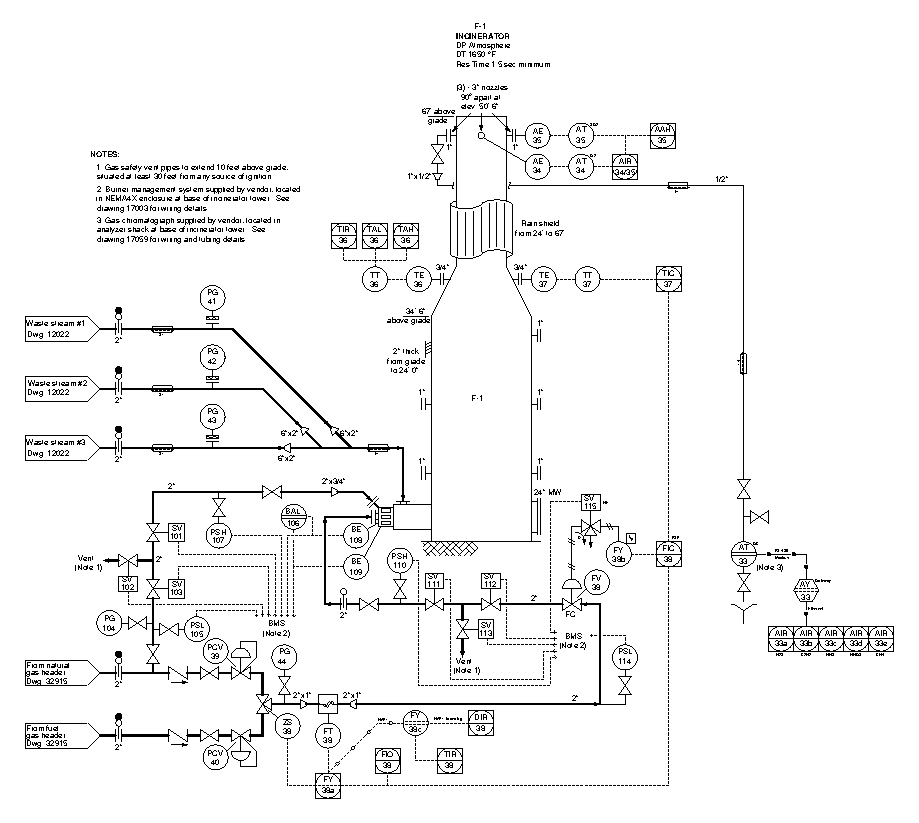
\includegraphics[width=15.5cm]{i0004rx01.eps}$$

Forklar hensikten med magnetventil SV-115, og angi om den er normalt energisert (NE) eller normalt spenningsløs (NDE).

\vskip 10pt

Forklar også hensikten med SV-111, SV-112 og SV-113 i dette kontrollsystemet.

\underbar{file i00951}
%(END_QUESTION)





%(BEGIN_ANSWER)

Magnetventil SV-115 avlufter all aktuatorluft fra flowventil FV-38 når spolen er spenningsløs. SV-115 er derfor ``normalt energisert'' for å opprettholde aktuatorluft til FV-38.

\vskip 10pt

SV-111, SV-112 og SV-113 hindrer at brenngass når brenneren når BMS sender tripsignal. SV-111 og SV-112 er {\it blokkventiler}, mens SV-113 er en {\it bleed}/avluftingsventil, altså en ``double-block and bleed''-løsning.

%(END_ANSWER)





%(BEGIN_NOTES)


%INDEX% Final Control Elements, valve: fail-safe solenoids
%INDEX% Process: incinerator (realistic P&ID shown)

%(END_NOTES)

